\newpage
\section{Ground penetrating radar}

\subsection{Principle}

Ground penetrating radar, or GPR, is a technology to investigate the subsurface using radars. A transmitter (in orange marked Tx on the figure \ref{fig:GPR}) generate a electromagnetic wave which is tranmitted in the ground via an antenna. This signal will propagate in the ground at different velocity depending of the material ($0.13 m/ns$ for sandstone or $0.5 m/ns$ for fresh water \cite{GPRAnalysis}) and will be both reflected and transmitted on the interface between to different materials. The reflected part will be received by the reception antena connected to the receiver (Blue marked Rx on the figure \ref{fig:GPR}).

\begin{figure}[h]
    \centering
    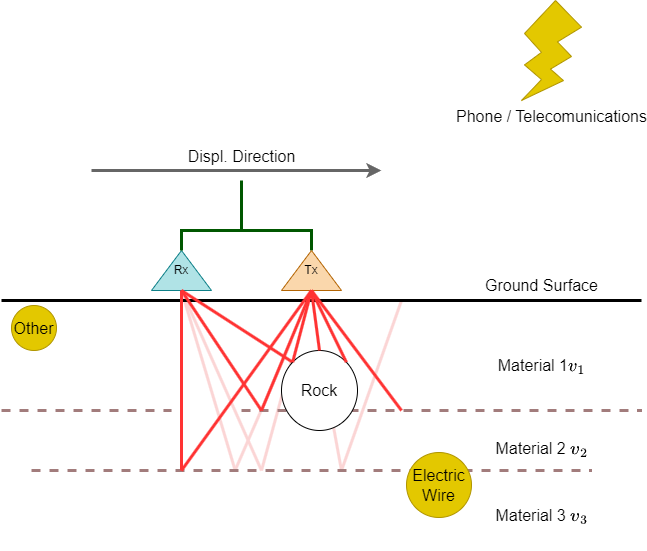
\includegraphics[width=0.8\linewidth]{Images/00_Theory/GPR Diagramm.drawio.png}
    \caption{Ground penetrating radar principle}
    \label{fig:GPR}
\end{figure}

Now we have the basic of the principle of GPR, we could consider different positioning for both antenna. Indeed, we could choose to keep the receiver fix and the transceiver moving, the opposite, both moving around a common mid point... In this report, we will only consider the usage where we have the transmitter and the receiver moving together, antenna perpendicular to the moving direction.
This usage of GPR permit to investigate a big area by doing multiple lines. On each lines, each measurement point will represent the ground under the GPR and so it will be possible to have an overview of the subsurface along the line. \cite{RnningGroundPerformance}

\subsection{Limitations}

As the GPR use a range of frequency from Mhz to Ghz which is also the range for many communication and electronics devices, GPR is very sensitive to all radio-electric perturbations. It must be operated far from any noise source as electric grid, GSM antenna...

An other limitation is that propagation characteristics depends of the material the electromagnetic wave propagate. It's to say that the energy lost by the wave during it's propagation depend on the material as well as the velocity. So for the same time windows\footnote{Time during the receiver is waiting the wave to come back before emitting a new signal. See \ref{SubSection:settings}}, if the signal propagate fast or slow will change the depth where we can see. Also, a material with a huge attenuation will limit the depth of the survey because the signal will lose very quickly the power.

Finally, every saline environment is almost impossible to investigate with GPR because the conductivity of salty water is very good, too good.

\subsection{Settings} \label{SubSection:settings}


\paragraph{Tension} The tension give an indication about the energy given to the emitted signal. Higher the tension is, deeper the signal will propagate but also higher the GPR will disturb the communication devices. The maximum tension allowed for civil survey is 400V even if in the past some GPR with a tension of 1000V was used. 

\paragraph{Frequency} The frequency is one of the most important parameter for a GPR survey because it's the frequency which define the resolution of the GPR. The figure \ref{fig:GPRFrequency} show that more precise will be the survey, less deep the penetration will be and higher the frequency will be needed. 

\begin{figure}[h]
    \centering
    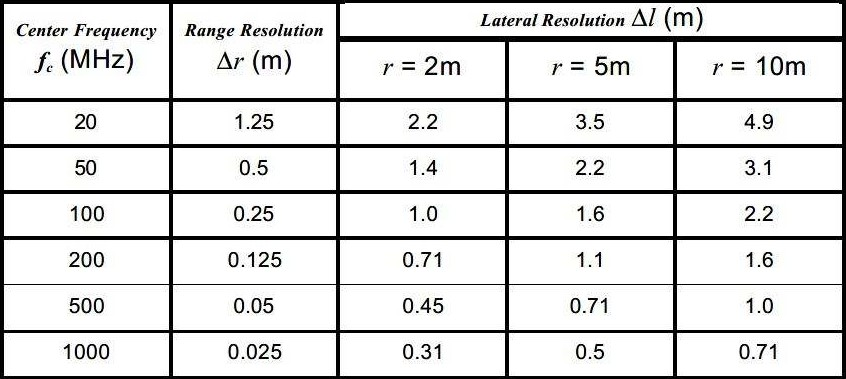
\includegraphics[width=0.6\textwidth]{Images/00_Theory/SS_FrequencyDepthResolution.jpg}
    \caption{Exemple of resolution length and depth versus frequency ($v=0.1m/ns$) from Sensor and Software \cite{UnderstandingDetection}}
    \label{fig:GPRFrequency}
\end{figure}

\paragraph{Number of stacks} The stacking consist to measure the same data many times to take the mediam or mean value and reduce the noise. The number of stacks should be the higher possible but will depend of the capabilities of the data-logger and of the different others parameters

\paragraph{Time windows} As defined before, the time windows is the time during which the receiver will wait the signal reflected in the ground. If we use a small time windows, we risk to missed some information. At the opposite, if the time windows is too large, the data logger will record only noise which will reduce the capability of the data logger.

\paragraph{Sampling interval}

\begin{figure}
    \centering
    \includegraphics{}
    \caption{Caption}
    \label{fig:my_label}
\end{figure}

\paragraph{Antenna separation}

\paragraph{Antenna orientation}

\paragraph{Sampling distance}

\paragraph{Velocity} The velocity is a secondary parameter for a GPR because in many cases the velocity is determined using GPR data. The important thing to know is that the velocity will convert the time windows into a depth windows and so determine the depth where the GPR is able to see.


